\documentclass[10pt,a4paper,danish]{article}
%% Indlæs ofte brugte pakker
\usepackage{amssymb}
\usepackage[danish]{babel}
\usepackage[utf8]{inputenc}
\usepackage{listings}
\usepackage{fancyhdr}
\usepackage{hyperref}
\usepackage{booktabs}
\usepackage{graphicx}
\pagestyle{fancy}
\fancyhead{}
\fancyfoot{}
\rhead{\today}
\rfoot{\thepage}

% Opsæt indlæsning af filer
\lstset{
  language=Python,
  extendedchars=\true,
  inputencoding=utf8,
  linewidth=\textwidth, basicstyle=\small,
  numbers=left, numberstyle=\footnotesize,
  tabsize=2, showstringspaces=false,
  breaklines=true, breakatwhitespace=false,
}

%% Titel og forfatter
\title{Informationsteknologi: Projekt e-læring \\ Projektkursus: Systemudvikling \\Forår 2011}
\author{Arinbjørn Brandsson (hkt789)\\Lasse Ahlbech Madsen (xsc606)\\Naja Mottelson (vsj465)\\Søren Pilgård (vpb984)\\
\\
Gruppeid : LO6\\
\\Instruktor: Lasse Nørregaard}

%% Start dokumentet
\begin{document}

%% Vis titel
\maketitle
\newpage

%% Vis indholdsfortegnelse
\tableofcontents
\newpage

%% HER STARTER RAPPORTEN
\section{IT-løsningens arkitektur og komponent-design}
Vores projekt består af en primært todelt løsning.
På overfladen har vi selve hovedprogrammet/klienten. Det er igennem dette at man gennemgår de konkrete forløb og bliver guidet igennem processen i at lave et spil. Nedenunder dette lag findes selve spillet.
\\

Vi har dog valgt at holde vores projekt åbent for i fremtiden at kunne udvide med flere forløb. Derfor består projektet i virkeligheden af tre dele:
\begin{itemize}
\item \textit{Hovedprogammet} der forklarer brugeren hvad han skal nu.
\item Et \textit{forløb} som klienten læser fra for at vide hvad brugeren skal. Forløbet er delt ind i en række trin med tilknyttede tests for at gøre det lettere for brugeren samtidig med der kan ydes skarpere kontrol med om brugeren har løst opgaverne undervejs korrekt.
\item Et \textit{spil} som er det konkrete produkt der arbejdes på af brugeren.
Spillet tilgås ikke gennem vores program men gennem brugerens eget tekstredigeringsværktøj.
\end{itemize}
På figur \ref{fig:brug_og_opdeling} ses hvordan brugeren bruger sit foretrukne tekstredigeringsværktøj til at tilføje og ændre på koden i spillet samtidigt med at vores værktøj bruges til at tilgå informationen om hvad brugeren skal foretage sig. Det er igennem de test der er tilknyttet trinene i forløbet at klienten kan holde styr på om brugeren kan få lov til at gå videre til næste trin.

\begin{figure}[h!]
  \begin{center}
    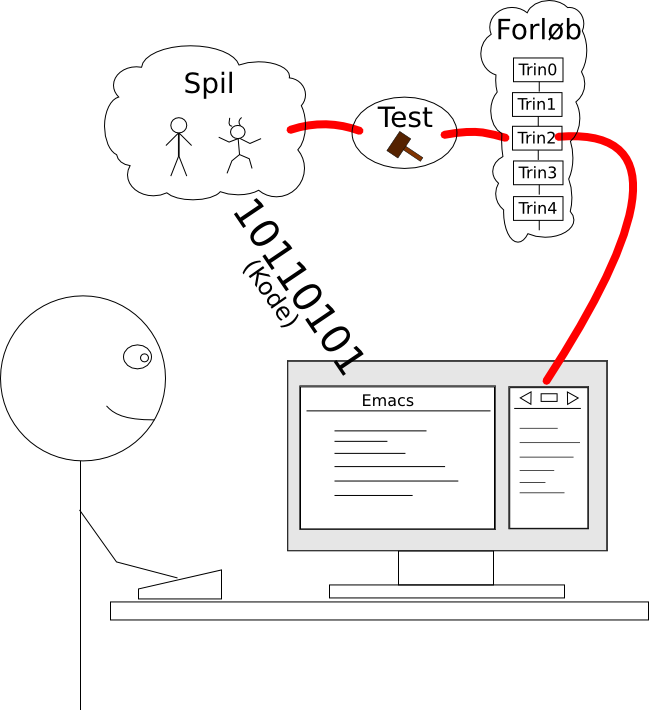
\includegraphics[scale=0.5]{afl3_brug_og_opdeling.png}
    \caption{Illustration af programmets brug og opdeling}
    \label{fig:brug_og_opdeling}
  \end{center}
\end{figure}


\paragraph{}
Da projektets primære opgave består i dets formidling, valgte vi at fokusere på selve spillet og forløbet til at starte med. klientens primære funktion består i at vise tekst samt at køre de tests der er defineret i forløbet. Uden et forløb med et tilhørende spil er klienten derfor nytteløst.
Vi startede derfor med at kode spillet inden selve klienten, for at vi så kunne begynde at lave forløbet. Vi har derfor på nuværende tidspunkt i projektet et stort set færdigudviklet spil men ikke noget af selve klienten på plads.

\subsection{Klienten}
Klientens primære funktion er at hente beskrivelser for opgaverne til hvert trin fra forløbet og vise det til brugeren. Derudover skal klienten køre de tests der er defineret til hvert trin når brugeren prøver at bevæge sig frem til det næste. Klienten vil derfor virke som en slags tynd fremviser der blot udfører hvad der er defineret i selve forløbet.

\begin{table}[h!]
  \begin{center}
    \begin{tabular}{llllll}
      \toprule
      Kriterium & Meget   & Vigtigt & Mindre  & Irrelevant & Trivielt \\
                & vigtigt &         & vigtigt &            & opfyldt  \\
      \midrule
      Brugbart        & &x& & & \\
      Sikkert         & & & &x& \\
      Effektivt       & & &x& & \\
      Korrekt         & & &x& & \\
      Pålideligt      & & &x& & \\
      Vedligeholdbart & & &x& & \\
      Testbart        & & & &x& \\
      Fleksibelt      &x& & & & \\
      Forståeligt     & &x& & & \\
      Genbrugeligt    & & &x& & \\
      Flytbarhed      & &x& & & \\
      Integrerbart    &x& & & & \\
      \bottomrule
    \end{tabular}
    \caption{Kvalitetsattributter for klienten.}
    \label{tab:kvalitetsattributter_program}
  \end{center}
\end{table}

\subsubsection{Kvalitetsattributter}
Dette afspejler sig også i kvalitetsatributterne som ses i tabel \ref{tab:kvalitetsattributter_program}.
Det er vigtigt at klienten er let at bruge så det ikke kommer i vejen for brugerens indlæring - det er meningen brugeren skal spekulere på hvordan han bedst muligt løser de stillede opgaver, ikke hvordan han bruger klienten.
Vi vil derimod ikke have behov for at tænke synderligt på hvor effektivt klienten er eller på hvor korrekt og pålideligt det er.
\\

Da systemet køres lokalt uden at skulle forbinde til diverse systemer behøver vi ikke at tænke på sikkerhed. Det eneste data der er at sikre, er de filer brugeren sidder og arbejder med. Vi anser det dog ikke vores opgave at sikre disse filer da de findes på lige fod med brugerens andre filer på det lokale system. Hvis programmet benyttes på en skole og der ønskes større sikkerhed bør brugerretigheder indføres på et bredere niveau der ikke har noget at gøre med vores program. Vi ønsker derfor ikke at sikre filerne på samme måde som f.eks. programmet Word heller ikke sikrer sine filer mod andre.
\\

Vi går heller ikke op i testbarheden af klienten da vi anser klienten for at være så lille at der ikke vil være behov for synderligt mange resurser her. Dette gælder dog kun for selve klienten. Når det kommer til forløbet og spillet er testbarheden et af de vigtigste punkter.
\\

Hvad vi tilgengæld går op i mht. klienten er fleksibilitet. Vi håber at kunne gøre klienten så minimal og generel at vi er i stand til at udvikle en bred palette af forskellige forløb med tilhørende spil som hver fører brugeren ind i forskellige emner med forskellige sværhedsgrader. Til at starte med satser vi kun på et enkelt forløb men vi håber med tiden at kunne udvide. Vi håber på at kunne bruge html eller et lignende format til at udtrykke tekst. Med html får vi en rig markup samtidig med vi kan indsætte referencer til hjemmesider samt billeder og lignende. Planen er at testene er skrevet som et pythonscript der køres, hvis testen returnerer en 'godkendt'-besked fortsætter klienten til næste trin, hvis testen fejler returnerer den derimod en fejlbesked med mulige hints om hvad brugeren kan have gjort forkert.
\\

Ved at gøre klienten minimal og generel gør man det samtidigt nemmere at genbruge koden i andre sammenhænge. Man kunne nok forholdsvist nemt konvertere programmet til andre typer opgaver eller måske andre programmeringssprog end python. Det er dog ikke noget vi anser som vigtigt på nuværende tidspunkt.
\\

Et andet punkt vi ser som vigtigt er forståelighed. Det er væsentligt at brugeren forstår hvad programmet gør samt hvad det vil have brugeren til at gøre så energien kan bruges på at finde den smarteste løsning på programmeringsopgaven.
Klienten skal helst være så transparent som muligt så brugeren kan fokusere på de vigtige ting.
\\

Flytbarhed er en vigtig ting da vi ikke ved præcis hvilken platform vores system bliver rullet ud på. Det kan være en skoles ældgamle it-systemer der kører windows 98, det kan være brugerens egen datamat der kører linux, eller måske en Mac.
Vi håber på at kunne ramme så bredt som muligt så flest muligt kan få gavn af vores program. Det er en af grundene til at vi udvikler i python da det er et sprog der er i stand til at køre på de fleste datamater. Samtidigt bruger alle i gruppen Linux sã derfor er det naturligt for os at sigte efter så brede løsninger som muligt. Disse tanker har vi især nu hvor vi er ved at beslutte os for hvilket GUI-bibliotek vi vil bruge til at udvikle klienten. Det skal helst være så nemt som muligt at installere, så vi vil gerne have så få afhængigheder (dependencies) som muligt.
\\

Sidst men ikke mindst har vi integrérbarheden som vi også vægter højt.
Da vi har valgt ikke at lave et indbygget tekstredigeringsværktøj, men at lade det være op til brugeren, er vi nød til at gøre det let at bruge sammen med eksisterende systemer. Det er derfor den grafiske del er designet som en lodret søjle så skærmpladsen kan deles med tekstredigeringsværktøjet så effektivt som muligt. Samtidigt er programmet designet meget minimalt med en rimelig genbrugelighed så man kunne forestille sig at klienten blev udviklet som f.eks. et emacs major-mode eller et visual studio/eclipse plugin.
\\

\paragraph{}

\subsubsection{Teknisk}
Rent teknisk regner vi med at bygge klienten i python med et af de mange gui biblioteker. Der findes en hel række af sådane biblioteker hvoraf det der hedder Tkinter er det som kan betegnes som standarden for python. Derudover findes PyGTK, PyQt samt wxPython som også er store og udbredte.
\\

Planen er at forløbet enten er en stor fil eller et filarkiv bestående af en række trin der hver har en beskrivelse samt en række pythonscripts der udgør testene. For at kunne lægge mere funktionalitet til beskrivelserne vil det være smart at benytte et allerede veldefineret format. Lige nu går tankerne på html da man der kan lave de fleste grundlægende ting så som understregninger, tabeller, henvisninger osv. Vi skal i så fald benytte et grafisk bibliotek der understøtter visning af simpel html.
Da testene er lavet i python vil det være trivielt at indlæse og afvikle dem.
\\

Man kan betragte løsningen som et simpelt Model-View-Controller setup.
Spillet og forløbet er det data der udgør modellen, klienten står for at køre de rigtige tests osv. i kontroldelen og det grafiske bibliotek står for at vise dette til brugeren.
\\

Dette er alt der er brug for til den tekniske løsning. Vi har ikke brug for at arbejde med mere avancerede databaser end hvad filsystemet tilbyder. Takket være de mange omfangsrige biblioteker behøver vi heller ikke at tænke på selv at skulle bygge teknologien til at vise tingene grafisk, hverken i klienten eller i spillet.

\subsection{Spillet}
\subsubsection{Teknisk}
Vi valgte at udvikle spillet i python primært fordi det er et lettilgængeligt sprog, både for os, men i lige så høj grad for brugerne. Samtidig havde vi gode erfaringer med biblioteket pygame som er i stand til at håndtere mange grundlæggene ting som tegning af billeder, håndtering af input fra brugeren osv.
\\

Som i klienten har vi også valgt at gå ud fra Model-View-Control mønstret da vi lavede spillet. MVC er et ret udbredt mønster i spilverdenen og vi har derfor valgt at følge det. 
Spillet selv er splittet op i en række forskellige moduler der tager sig af forskellige ting. Vi har valgt at være ret agressive med opdelingen, dels for at gøre det mere overskueligt for brugeren og dels for at vænne dem til at dele deres kode mere op. Opdelt kode er lettere at overskue, rette og teste - tre ting vi gør brug af i projektet.

Spillet består af følgende filer:
\begin{itemize}
\item \textit{game.py} indeholder \"main\" metoden, det er herfra spillet startes. Derudover indeholder den selve spilløkken.
\item \textit{model.py} indeholder alle de klasser der er i spillet, her er alle spilobjekterne defineret.
\item \textit{data.py} er en slags database over alt i spillet. Modulet holder styr på de forskellige spilkonstanter så som vinduestørrelsen, samt sæt af spillets objekter. Når et nyt objekt bliver oprettet skal det tilføje sig i de relevante grupper så de bliver opdateret og vist korrekt.
\item \textit{mapping.py} banerne til spillet består af simple tekstfiler der indlæses og gemmes i data modulet. Når banerne er blevet indlæst er der funktionalitet i mapping modulet der kan omsætte banen til faktiske objekter.
\item \textit{direction.py} Udgør enums for alle 4 verdenshjørner, modulet bliver brugt til bevægelse af spilleren.
\item \textit{functions.py} indeholder lidt blandede funktioner.
\item \textit{resources.py} indeholder alt funktionalitet der har med faktisk indlæsning af data at gøre.
\end{itemize}

Udover disse filer findes to mapper \textit{images} som indeholder alt billedmaterialle, samt \textit{maps} der indeholder banefiler.


\begin{table}[h!]
  \begin{center}
    \begin{tabular}{llllll}
      \toprule
      Kriterium & Meget   & Vigtigt & Mindre  & Irrelevant & Trivielt \\
                & vigtigt &         & vigtigt &            & opfyldt  \\
      \midrule
      Brugbart        & & &x& & \\
      Sikkert         & & & &x& \\
      Effektivt       & &x& & & \\
      Korrekt         &x& & & & \\
      Pålideligt      &x& & & & \\
      Vedligeholdbart & &x& & & \\
      Testbart        &x& & & & \\
      Fleksibelt      &x& & & & \\
      Forståeligt     & &x& & & \\
      Genbrugeligt    & &x& & & \\
      Flytbarhed      & &x& & & \\
      Integrerbart    & & & &x& \\
      \bottomrule
    \end{tabular}
    \caption{Kvalitetsattributter for Spillet.}
    \label{tab:kvalitetsattributter_spil}
  \end{center}
\end{table}

\subsubsection{Kvalitetsattributter}
Vi valgte også at udarbejde et skema af kvalitetsatributter for spillet da kode opgaven deri på mange måder er mere omfattende end klienten. Samtidig er spillets fokus og klientdelens fokus så forskellige at det gav god mening at kigge nærmere på hvor vores data og klient adskilte sig fra hinanden. I tabel \ref{tab:kvalitetsattributter_spil} ses resultatet.
\\

Det ses at brugbarheden er mindre vigtig i forhold til klientens. Dette er et aktivt valg fra vores side. Vi vil i dette spil fokusere mere på at få noget frem på skærmen som brugeren kan inteargere med og udvide, end at få det til at være særligt brugervenligt. Vi har derfor valgt f.eks. ikke at lave menuer, spillet starter direkte ind i den valgte bane og spilleren dør slutter spillet automatisk.
Det er ting som er væsentlige hvis man gerne vil tjene penge på et velpoleret spil, men det er ligegyldigt hvis man bare vil lege og lære.
\\

Sikkerheden er irrelevant, idet der ikke er nogen nødvendig kontakt til andre systemer. I og med at det er brugeren selv der udvikler spillet vil det heller ikke give mening at beskytte spillet mod snyderi fra vores side, så der er intet spildata der skal beskyttes.
\\

Effektiviteten af spillet er dog lidt vigtig: hvis spillet skal køre med 30fps har man 33 millisekunder til at håndtere input, udføre spillogikken samt tegne spillet. Dog er pygame istand til at håndtere selve tegnefunktionaliteten hvilket er implementeret i c og foregår forholdsvist stærkt så vi slipper for at skulle tage os af det manuelt.
\\

Det er vigtigt at koden er korrekt og pålidelig, på den måde er vi istand til at lave langt mere gennemførlige tests af brugerens spil. Dermed kan vi sikre os at brugerne lærer det de skal.
\\

Vedligeholdbarheden er også vigtig, den er med til at gøre det nemmere for brugeren at rette sine fejl og komme videre i forløbet. Vedligeholdbarhed kan blandt andet opnås ved at gøre koden nemmere at overskue.
\\

Testbarheden skal være i top så vi kan udføre de tests vi skal for at lade brugeren gå videre til næste trin.
\\

Fleksibiliteten er prioriteret højt da det gør det nemmere for brugeren at modificere spillet til hans behag. På den måde bliver det brugerens spil istedet for vores. Hvis brugeren knytter sig til spillet er der større sansynelighded for at brugeren fortsætter og for mere ud af forløbet. Samtidigt kan det være at det giver brugeren blod på tanden til at kigge nærmere på spiludvikling.
\\

Det er vigtigt at forståeligheden er høj da det er meningen brugeren skal lære så meget som muligt. Derfor vil vi også forsøge at pakke de mere pygame specifike ting væk så brugeren kan fokusere på det væsentlige.
\\

Genbrugeligheden bør være høj på to måder, dels er det vigtigt at brugeren kan tage de teknikker han har lært gennem forløbet med sig, dels vil det være en fordel hvis han kan udnytte segmenter af koden hvis han har lyst til at udvikle sit eget spil.
\\

Igen er det vigtigt med flytbarheden, brugeren skal ikke kun kunne afvikle klienten men også sit spil på den platform han sidder ved.
\\

Integrerbarheden er til gengæld forholdsvis ligegyldig i denne sammenhæng, da spillet bare skal kunne køre selvstændigt.



\section{Erfaringer med evalueringer af IT-løsningen i samarbejde med brugerne}
Denne sektion er en smule besværlig for vores gruppe at skrive, eftersom vi på nuværende
tidspunkt ikke har en kørende prototype af vores program som kan afprøves af brugerne. 
Som beskrevet i de hidtidige rapporter kommer vores program til at bede brugeren om at kode
et bestemt spil - siden Delrapport 2 har vi brugt vores tid på at implementere dette spil.
Vores motivation til at prioritere på denne måde er at det (fra vores synspunkt) vil være
umuligt at implementere de enkelte trin i undervisningsforløbene hvis man ikke har et 
solidt kendskab til spillets tiltænkte struktur.  

\subsection{Problematikker ifbm. afprøvning}
Dette er en problematisk situation: eftersom vores program beskæftiger sig med pædagogik
er netop afprøvning med brugere en central del af udviklingen. Dog: i forbindelse med dette 
projekt er vores spil nærmere at betragte som data end som 
programmel, og det er ikke selve spillet der skal afprøves af brugerne.

I vores arbejde har vi fundet frem til to essentielle udfordringer mht. afprøvning, som præger 
vores projekt i en smule højere grad end normalt. Først og fremmest vurderer vi at det potentielt 
er sværere for os at lave traditionel løbende afprøvning, eftersom vores 
program ikke rigtig lader sig opdele og afprøve separat. Det er derfor en smule besværligt at 
sikre en optimal iterativ afprøvning i det hele taget. 

Mere vigtigt end dette er dog hvad man kan kalde forudsætningerne for vores program - selve den
måde interaktionen er planlagt er simpelthen problematisk at teste, eftersom en typisk use case
vil vare betragteligt længere end fx. use casen for et af de databaseadministrationssystemer der
præsenteres i lærebogen. Et læringsværktøj er jo netop et program man forventes at bruge som
minimum nogle timer på at arbejde med, og dette har vi ikke resurser til at afprøve i gruppen. 
En anden, mere praktisk del af denne problematik er at vores tilgængelige brugergruppe muligvis er 
uegnet til at give et repræsentativt resultat. Vores ønske med programmet er at skabe et læringsværktøj
som kan benyttes af folk på et forholdsvis lavt niveau af programmeringserfaring, men det kræver
dog kendskab til bl.a. grundlæggende python-syntaks (en tillæringsopgave som ikke er triviel for
mange førstegangsprogrammører). Den datalogiklasse vi samarbejder med har ikke modtaget undervisning
i python, så de eneste af dem vi ville kunne benytte som testpersoner ville være dem der kunne 
overtales til at sætte sig ind i grundlæggende python på egen hånd, eksternt fra undervisningen. 
De elever der ville være villige (og i stand til) dette er sandsynligvis mere engagerede og dygtigere
end normen, og ville således ikke give et helt troværdigt indblik i de spørgsmål vi kunne tænke os
at få besvaret. 

Med baggrund i disse overvejelser har vi derfor besluttet at følge en lidt anderledes afprøvningsstrategi,
som dokumenteres i dette afsnit. 

\subsection{Overvejelser vedr. brugertests}
Som det kan ses af billeddokumentationen i sidste rapport, kommer den grafiske brugergrænseflade
for vores program til at være meget simpel. Endvidere føler vi selv at vi har et godt
billede af hvordan den skal udformes fra papir-mockup-testingen som beskrives i Delrapport 2.
Vi mener derfor ikke at det GUI-specifikke egentlig er af største vigtighed når det kommer til bruger-afprøvning. 
Hvad der derimod er kritisk at afprøve er udformningen af de forskellige trin vi har opdelt 
kodeopgaverne i - om niveauet er for højt/lavt, om opgavebeskrivelserne fungerer, om rækkefølgen
er intuitiv mm. 

\subsection{Planlægning af brugertests}
I vores kommende afprøvningsarbejde er vi, som nævnt, nødt til at overvinde den forhindring at en
kørende prototype mangler. Måden vi regner med at gøre dette kan siges at være en variation over 
sidste rapports mockup-testing: I stedet for at give testpersonerne et stykke programmel imellem 
hænderne agter vi at sætte os ned med dem og 'snakke' de forskellige opgaver igennem. Eftersom denne
form for testing sandsynligvis kommer til at kræve en del arbejde fra hvert gruppemedlem (vi regner
fx. med at have én person som er ansvarlig for interaktion med testpersonen og én som er ansvarlig 
for at dokumentere processen) regner vi med at nøjes med at udføre afprøvning med 2-3 elever fra 
datalogiklassen på Greve gymnasium. Dette afhænger dog også af hvor mange elever der viser sig at 
være interesserede i at deltage. 

Måden vi planlægger at udføre selve afprøvningen er ved at sætte os ned med den enkelte elev
og formulere de individuelle kodeopgaver for dem. Derefter vil vi bede dem beskrive (et bud på)
den algoritme de kunne forestille sig at benytte for at løse den. Der er selvfølgelig en del 
problematikker iboende i denne måde at gøre det på: En datalogisk uerfaren gymnasieelev kan 
sandsynligvis ikke forventes at være vant til at skulle komme med et bud på datalogisk problem-
løsning 'med det samme' på denne måde, og måske vil de have svært ved at forholde sig til den
måde at tænke på. En anden ting vi er nødt til at tænke på er at der sandsynligvis er en forskel
på hvor nemt testpersonerne vil have ved at udføre opgaven alene og med god tid, og under tidspres
med universitetsstuderende der observerer dem imens. 

Der er dog også visse fordele ved denne måde at udføre afprøvningen af programmet (eller, 
mere præcist, af programmets datalogiske indhold). Problematikken i at ingen af vores 
forsøgspersoner har specifik erfaring med python kommer her ikke til at udgøre et problem, 
eftersom de ikke bede kode så meget som at udtrykke sig i generelle algoritmiske termer. 

\section{Projektsamarbejdet}
Siden sidste aflevering har vi holdt pause i påskeferien, og har derfor kun haft to uger til at holde møder og arbejde. Herefter har vi holdt jævnlige møder, hvor vi har uddelegeret, prioriteret og planlagt den videre udvikling af projektet og rapportskrivningen. 

Vi oplever visse kommunikationsproblemer i gruppen; folk er dårlige til at melde ud om status på deres opgaver, hvilket er aldeles problematisk. Det begrænser vores overblik over den hidtidige udvikling af projektet. Man kan ikke hjælpe dem, hvis de sidder fast, da de ikke melder ud om dette. Er de overhovedet i gang? Er der andre, som bliver nød til at overtage opgaven? Eller er den måske næsten færdig? I sidste ende lægger det pres på resten af gruppen og er med til at skabe interne konflikter. For at løse dette har vi forsøgt os med alvorlige samtaler med de medlemmer af gruppen, som opfører sig sådan. Vi håber at det vil være nok, da vi ellers ikke kan se, hvad de skal gøre for at forbedre situationen. Ydermere er der en tendens til at tage lidt for let på tidsfrister, i særdeleshed i forbindelse med opgaver som rapportskrivning. Ting bliver lavet meget sent, og det er svært for den ansvarshavende at nå at læse det igennem og give kritik. I sidste ende står vi med et dårligere produkt. For at løse dette har prøvede vi efter sidste raportaflevering at uddelegere opgaverne tidligere, så folk havde længere tid til at lave dem. Dette var dog ikke synderligt effektivt, så selvom vi regner med at vedblive med at uddelegere tidligt vil vi prøve at finde andre måder at løse problemet. Som et fremtidigt eksperiment, forsøger vi at uddelegere opgaver parvis. Det vil sige at en enkelt person får ansvaret for at en given opgave bliver lavet, mens den anden søger for at følge processen, og hjælper med sørge for at den ansvarshavende ikke går død i det.

\subsection{Mødeform og dokumentationsstrategi} 
Til interne møder holder vi os stadig til en ret basal referatstrategi, hvor vi noterer beslutninger og statusopdateringer ved de enkelte punkter i dagsordenen og konkrete forslag og tanker ved diskussioner. Dette er praktisk på kort sigt, men det giver ikke en den store indsigt i, hvorfor vi har taget de beslutninger vi har, og kan i værste fald være unyttige i en eksamenssammenhæng, når vi skal redegøre for processen. Dette er stadig et punkt vi forsøger at forbedre, men det er ikke prioriteret særligt højt i forhold til mere nærværende opgaver. Rapporterne tager meget tid, og vi er ikke så langt med selve it-projektet, som vi gerne ville være. Konsekvensen af dette er, at vi ikke kan finde tid til at udbedre den mangel, og fortsætter med halvtilstrækkelige referater. Referaterne deler vi over Github (sammen med vores kode), og er derved let tilgængelige for alle gruppemedlemmer. Dette er vi glade for, om end vi har problemer med, at det ikke er alle, der har lige nemt ved at finde ud af git.

Vores møder foregår som regel med stramme dagsordener, der er med til at effektivisere dem, og minimere spildtid. Vi udpeger en referent, og går punktvist frem. Der er for det meste fuldt fremmøde, men vi spilder en betragtelig mængde tid på, at folk kommer for sent. For at udbedre situation forsøger vi at lægge møderne i forlængelse af forelæsninger og øvelsestimer, så folk allerede er her. Herudover har vi på det seneste oplevet problemer med sygdom, og vi mangler ofte en person. Dette er der selvfølgelsig ikke en helt masse at gøre ved, men vi forsøger at opfordre folk til overveje, om de nu også har det SÅ dårligt, og måske kunne komme alligevel.


\subsection{Projektstyring og implementation}
Som nævnt i prototypeafsnittet, så har vi ingen kørende prototype. Dette er ikke uproblematisk, men vi har valgt at fokusere på at lave den pædagogiske del af projektet først. Dette har vi gjort fordi programmet i sig selv er meget simpelt, og ikke rigtig kan testes alene, ej heller ville det give mening at teste det mere, end vi allerede har gjort med vores papirsprototyper. Programmet drejer sig i høj grad om indholdet af forløbene, og uden nogen forløb er programmet tomt og ubrugeligt. Derfor har vi valgt at udvikle det første forløb først eller evt. en del af det, så det kan testes. Denne del af programmet, kan også håndkøres, og er egnet til testing.

Som nævnt i den tidligere rapport havde vi et problem med, at det meget var en enkelt person, der stod for ansvaret for det hele. Dette var ikke udelukkende problematisk, fordi denne person stod med en væsentlig arbejdsbyrde, men også grundet dataindkapsling. Det var kun den ene person, som havde et egentlig overblik over opgaven. Dele af projektet var der ikke andre, som tog del i, og dermed havde resten af gruppen ikke rigtig noget indblik i det. Dette er stadig et problem i gruppen. Vi har ikke haft tid til at fokusere på omlægning af arbejdsstrukturen, og finder os derfor stadig i samme situation. 

For at øge kontrollen med projektet og sikre at vi får det hele med, har vi uddelt 4 af hovedansvarsområderne i projektet til en person hver. Disse er projektledelse, kodeudvikling, unit-tests og dokumentation af kode. Tanken er ikke, at hver enkelt person står for sit punkt alene, men vedkommende har ansvaret for, at det bliver gjort og har opsyn med punktets status. På denne måde aktiverer og engagerer vi også alle gruppemedlemmer, så ansvaret ikke hænger på blot en del af gruppen, som det ellers har været præget af tidligere i projektet. Ydermere har vi fordelt de første trin i vores program, så vi hver især skriver udkast til 2-3 af trinene i vores første forløb. Dog skal alle kigge på samtlige punkter - dette er gjort fordi punktet i høj grad omhandler pædagogik, og man kan forestille sig ret forskellige tilgangsvinkler til dette. Ved at splitte det op sikrer vi, at vi får alles forslag til formidlingen, og kan i fællesskab finde en optimal løsning, hvor vi bruger de bedste dele fra de enkelte vinkler. En anden vigtig grund er selvfølgelig ansvarsfordeling, hvor vi sørger for at alle laver noget, og det ikke bliver en delmængde af gruppen, som kommer til at stå for det hele.  

Vi er kommet ordentligt i gang med selve projektet nu, der har ellers hængt lidt, og blevet nedprioriteret i forhold til rapportskrivningen. På trods af begrænset tid, går det relativt hurtigt fremad, og vi regner med at kunne have i hvert fald en kørende prototype ved kursets slut, om end ikke helt så omfattende, som vi kunne have ønsket. 


\section{Reviews}
\subsection{User Testing, Discount User Testing, af Rolf Molich}
Artiklen handler om usability testing, (User testing), hvordan man holder en vellykket brugertest, samt hvordan man sørger for at  testbruger føler sig godt tilpas før, under og efter en brugertest, samt forskellige teknikker man kan tage i brug. Artiklen beskriver for det meste en testprocedure, kaldet "Thinking Aloud Testing", hvor testbrugeren siger højt hvad det er han tænker mens han bruger programmet, (ting som hvad han er i tvivl om, hvordan han forventer at programmet reagerer, og hvordan han fortolker en besked). Disse ting bliver enten skrevet ned af en tester, eller optaget på video eller på lydbånd.

En "Thinking Aloud Testing" kræver dog forberedelse. Først skal man tjekke om testbrugerne er over- eller under-kvalificeret ved at interviewe dem på forhånd, (dog dette behøves ikke for vores brugertest, da vi låner nogle gymnasie elever som læser datalogi til at teste programmet siden de ligger i vores målgruppe). Siden skal man også lave en liste af opgaver som testbrugerne skal løse, hvor den første opgave skal være en nem opgave som kan løses på få minutter, så at testbrugerne ikke bliver stresset eller nervøse. Denne liste af opgaver er en integreret del af vores hjælpeprogram, og derfor vil en del af vores brugertest gå ud på at se om hvis testbrugerne kan forstå disse opgaver. Det er også en god idé at afslutte en brugertest med en debriefing, hvor man taler med testbrugeren, og finder ud af hvilken tanker de havde om programmet, hvad var godt ved programmet, og hvad man kunne gøre bedre eller formulere bedre. En vigtig del under debriefing er at man behandler testbrugernes foreslag med respekt, for ellers vil de være tilbageholdende med foreslag og meninger omkring projektet.

Artiklen gennemgik også kortvarigt en anden test procedure, "Constructive Interaction", hvor man lod to testbrugere arbejde sammen for at kunne løse opgaverne, hvorefter de vil diskutere programmet, hvad det gjorde godt, og hvad kan laves om. Vi vælger dog at ikke tage denne test procedure i brug, eftersom vores testbrugere er gymnasieelever vil de sikkert bruge tiden ukonstruktivt, og ikke tage deres opgave seriøst.

Brugertest er afgørende for vores projekts success. Da vores program er et hjælpeprogram, designet til at lære gymnasieelever til at kunne kode spil i python, skal de instruktioner og opgaver som programmet viser frem til brugeren være klare og nemme at forstå. Derfor passer "Thinking Aloud Testing" rigtig godt til vores projekt - ved brug af denne teknik kan vi, fra vores kunder, høre hvad det er de forventer programmet skal kunne gøre, samt om hvis nogle af vores hints, opgavespecifikationer eller meddelser er uklare, eller ikke fortæller nok om opgaven. Artiklen gav også tips til god etikette før, under og efter en brugetest, hvilket kommer til at være meget nyttige for os, da vores testbrugers input er uhyre vigtigt for os.

Ikke kun det, artiklen vil også hjælpe os med at skrive de trin som vores fremtidige brugere skal gennemføre - artiklen gav gode råd som, for eksempelt, det første trin skal være det nemmeste så at testbrugerne ikke ville føle sig frustreret eller gå i panik hvis de ikke kan løse det første trin. Man kan vel sige at artiklen gav os gode pædagogik råd, hvilket er præcist det som vi har brug for til vores projekt. Derfor kan man sige at artiklen gavner vores gruppe både før vores brugertest, samt efter vi har holdt vores brugertest.

\subsection{Software Architecture in Practice, af Bass, Clements og Kazman}
Artiklen handler om software architecture, hvor software architecture er systemets struktur, eller strukturer, som omfatter sofware elementer, og de relationer imellem elementerne, samt de antagelser som elementer kan have om andre elementer. Arkitekturen definere softwarets elementer, og omfatter de offentlige dele af softwaret. Et arkitektur består af strukturer, (dette plejer at være i flertal medmindre softwaret er meget specialiseret eller simpelt), og disse strukturer behøver ikke at være af samme type, da strukturerne forventes at dække over alle dele af systemet.

Strukturerne for vores program regnes at være af én slags - en modulær baseret struktur, (hvor systemet kan splittes i mindre dele), da dette passer bedre for vores projekt. Siden at hovedparten af vores projekt består af trin, som består af mindre trin, kan denne form af struktur passe godt til systemet, siden at dette lader systemet blive brudt ned i mindre dele. Og siden hvert del af disse trin behøver et overordnet trin for at kunne udføres, (et trin har 'checkpoints', som derefter har hints), sørger denne slags struktur for at systemet bliver sådan.

Derfor kan det være at det bedste form for struktur for vores system ville være at bruge et 'logical' struktur, hvilket opfylder det basis som udgør et modulært struktur. Desværre gav artiklen ikke en bedre beskrivelse af hvad et logical struktur er, udover at det er modulært, og består af objekter, så det kan godt være at det ikke er lige så perfekt som vi tror det er. Men ud fra hvad artiklen har fortalt, virker det godt for os.

De andre former for strukturer som artiklen fortalte om virkede som om de ikke ville fungere for vores system, og derfor vil vores system kun have et struktur. Man kan måske bruge et 'physical' struktur, men da vi lader et tredje-parti program processere koden, samt vi ikke rigtig har brug for meget kommunikation imellem elementerne, kan det nok være at det bare ville komplicere ting at have det med.

Da vi, i gruppen, har haft problemer med at kommunikere med hinanden om hvor vi står med vores arbejde, hvad vi skal gøre med vores dele af rapporten, m.m., vil et arkitektur hjælpe os som en gruppe, da et arkitektur vil stå som en basismodel for det system som vi skal lave. Ved at have en basismodel stående fremme, vil vi alle samme vide hvor i projektet vi står, og det vil gør det nemmere for os holde os organiseret - noget som gavner alle grupper. Og hvis der opstår uenigheder eller misforståelser omkring vores opgaver, vil et arkitektur hjælpe os videre.

\subsection{Foundations for the Study of Software Architecture, af Perry, D. og Wolf, A}
Artiklen fortæller om en anderledes form for software architecture end præsenteret. Artiklen påstår at et systems arkitektur består af tre dele: 
\begin{enumerate}
\item Elementer,
\item Form, (Elementernes begrænsninger), og
\item Basis for systemet, (dette plejer at være systemets krav).
\end{enumerate}
Dette er en temmelig stor forskel. Bass, Clements og Kasman påstår at systemets arkitektur består af mange forskellige strukturer, som så kollektivt beskriver systemets arkitektur, hvorimod Perry og Wolf ser arkitektur som tre kriterier som bliver defineret, samt det er forventet at arkitekten arbejder med kunden for at kunne definére systemets arkitektur. 

Dette fører til et problem: Hvilken form for system arkitektur er så bedre at bruge for vores projekt? Umiddelbart vil vi sige at den form for system arkitektur beskrevet i Foundations for the Study of Software Architecture ville være af større gavn for vores system. Hvis vi skulle tegne op alle de strukturer som kan beskrive vores system, ville vi ende med ikke særlig mange, hvilket modarbejder Bass, Clements and Kazmans system arkitekturs styrke - ved at have mange forskellige strukturer, vil arkitekturen kunne beskrive systemet på mange flere måder end hvis man havde meget få strukturer. Dog for mindre projekter, som kræver at man arbejder mere intimt med sin kunde, vil Perry og Wolfs arkitektur form være bedre for vores system.

Noget andet som artiklen diskutere er Process/Data/Connector Interdependence. Dette er navnet som artiklen giver et fænomen hvor når man laver arkitekturen, er det vigtigt at man har forskellige synspunkter i arkitekturen. Artiklen fortæller om at forarbejdning, data og forbindelser alle har en effekt på hinanden, så hvis et synspunkt er fastsat, (for eksempel hvis forarbejdningens synspunkt er givet), vil der blive givet fokus på datastrømmen igennem forarbejdningens elementer. Det som dette betyder er at arkitekturen skal kunne give et overblik på alle dele af systemet, samt at hvis man kigger på den del af systemet, skal man kunne se hvordan den relatere sig til andre dele af systemet. 

Siden en stor del af vores program er datastrømmen imellem vores hjælpeprogram og det text editor som brugeren kommer til at vælge, samt forarbejdningen af disse dataer, er dette punkt meget hjælpsomt for os. Ved at få et overblik over hvordan de forskellige dele af vores program virker, vil vi nemmere kunne se, via vores system arkitektur, hvilken dele af systemet er afhængige på hvilken andre dele af vores system.
\end{document}
